% Standalone render of the architecture diagram for the README.
% Build: pdflatex architecture_standalone.tex, then rasterize (see docs/scripts/render_architecture.py).
\documentclass[border=8pt]{standalone}
\usepackage[T1]{fontenc}
\usepackage[utf8]{inputenc}
\usepackage{libertinus}
\usepackage{libertinust1math}
\usepackage{amsmath}
\usepackage{xcolor}
\usepackage{tikz}
\usetikzlibrary{arrows.meta,positioning,fit,backgrounds,calc,shapes.geometric}
\definecolor{ink2}{HTML}{52514E}
\definecolor{rulec}{HTML}{C3C2B7}
\definecolor{deep}{HTML}{163A6B}
\definecolor{panel2}{HTML}{F7F6F2}
\definecolor{statec}{HTML}{2A78D6}
\definecolor{queuec}{HTML}{EB6834}
\definecolor{odmec}{HTML}{1BAF7A}
\definecolor{physc}{HTML}{6250D6}
\newcommand{\SFD}{S_{\mathrm{FD}}}
\newcommand{\SLWR}{S_{\mathrm{LWR}}}
\begin{document}
% Shared by main.tex (Section 4) and architecture_standalone.tex (README image).
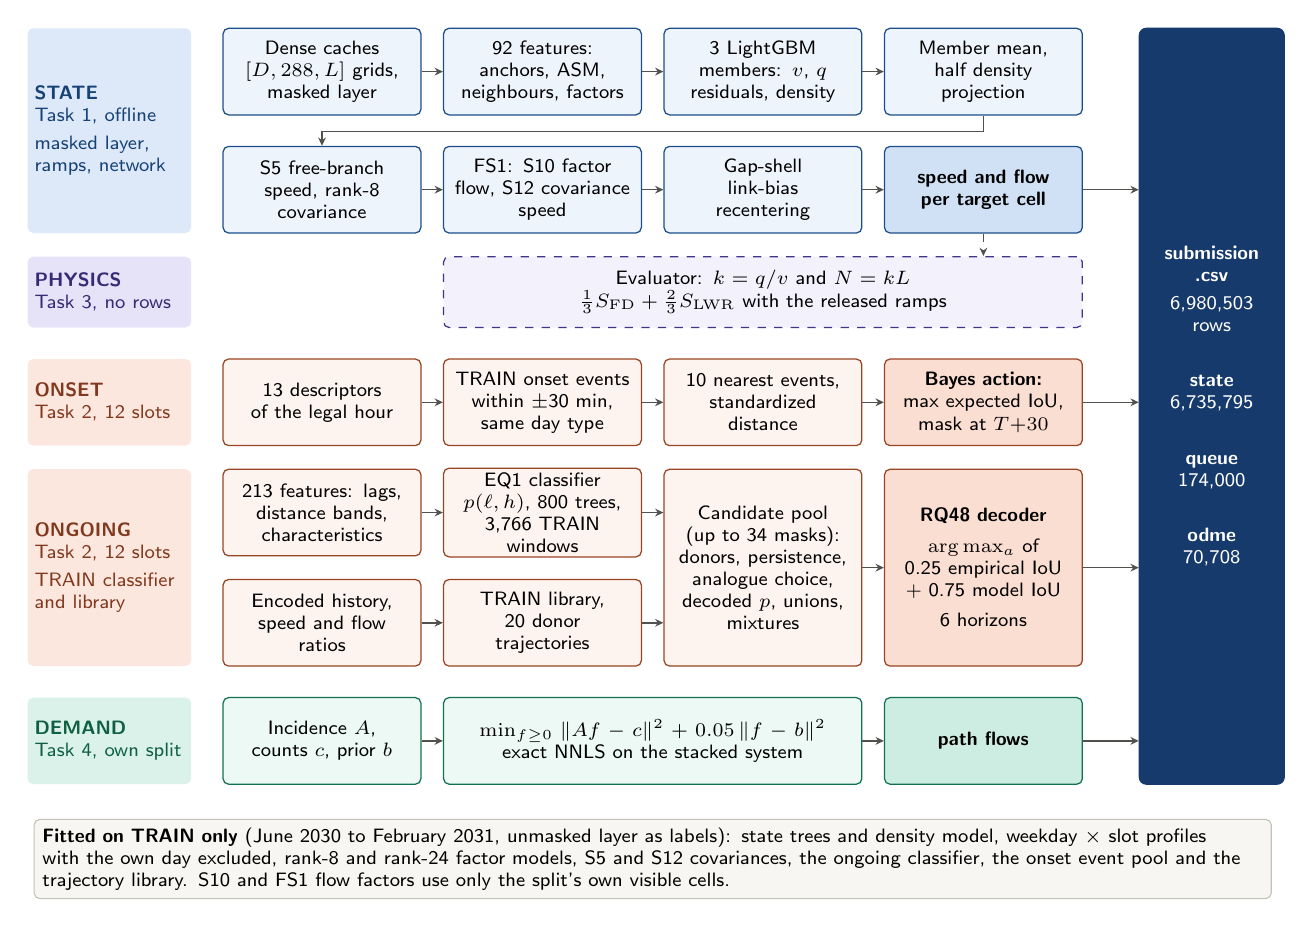
\begin{tikzpicture}[x=1mm,y=1mm,font=\sffamily\scriptsize,
  every node/.append style={execute at begin node={\hyphenpenalty=10000\exhyphenpenalty=10000}},
  stage/.style={draw=#1!65!black,fill=#1!8,rounded corners=2pt,align=center,inner sep=1.6pt,
                text width=24mm,minimum height=11mm,line width=0.45pt},
  lab/.style={draw=none,fill=#1!16,rounded corners=2pt,align=left,inner sep=2.5pt,text width=19mm,
              font=\sffamily\scriptsize,text=#1!55!black},
  arr/.style={-{Stealth[length=3pt,width=2.8pt]},line width=0.55pt,color=ink2},
  darr/.style={-{Stealth[length=3pt,width=2.8pt]},line width=0.55pt,color=ink2,dashed}]

% lane labels
\node[lab=statec,minimum height=26mm] at (11,-7.5) {\textbf{STATE}\\Task 1, offline\\[2pt]masked layer,\\ramps, network};
\node[lab=physc,minimum height=9mm] at (11,-28) {\textbf{PHYSICS}\\Task 3, no rows};
\node[lab=queuec,minimum height=11mm] at (11,-42) {\textbf{ONSET}\\Task 2, 12 slots};
\node[lab=queuec,minimum height=25mm] at (11,-63) {\textbf{ONGOING}\\Task 2, 12 slots\\[2pt]TRAIN classifier\\and library};
\node[lab=odmec,minimum height=11mm] at (11,-85) {\textbf{DEMAND}\\Task 4, own split};

% state
\node[stage=statec] (s1) at (38,0)   {Dense caches\\$[D,288,L]$ grids,\\masked layer};
\node[stage=statec] (s2) at (66,0)   {92 features:\\anchors, ASM,\\neighbours, factors};
\node[stage=statec] (s3) at (94,0)   {3 LightGBM\\members: $v$, $q$\\residuals, density};
\node[stage=statec] (s4) at (122,0)  {Member mean,\\half density\\projection};
\node[stage=statec] (s5) at (38,-15) {S5 free-branch\\speed, rank-8\\covariance};
\node[stage=statec] (s6) at (66,-15) {FS1: S10 factor\\flow, S12 covariance\\speed};
\node[stage=statec] (s7) at (94,-15) {Gap-shell\\link-bias\\recentering};
\node[stage=statec,fill=statec!22,font=\sffamily\scriptsize\bfseries] (s8) at (122,-15) {speed and flow\\per target cell};
\draw[arr] (s1) -- (s2); \draw[arr] (s2) -- (s3); \draw[arr] (s3) -- (s4);
\draw[arr] (s4.south) -- ++(0,-2) -| (s5.north);
\draw[arr] (s5) -- (s6); \draw[arr] (s6) -- (s7); \draw[arr] (s7) -- (s8);

% physics
\node[stage=physc,text width=80mm,minimum height=9mm,dashed] (p1) at (94,-28)
  {Evaluator: \mbox{$k=q/v$} and \mbox{$N=kL$}\\\mbox{$\tfrac13\SFD+\tfrac23\SLWR$} with the released ramps};
\draw[darr] (s8.south) -- (s8.south |- p1.north);

% onset
\node[stage=queuec] (o1) at (38,-42) {13 descriptors\\of the legal hour};
\node[stage=queuec] (o2) at (66,-42) {TRAIN onset events\\within $\pm$30 min,\\same day type};
\node[stage=queuec] (o3) at (94,-42) {10 nearest events,\\standardized\\distance};
\node[stage=queuec,fill=queuec!22] (o4) at (122,-42) {\textbf{Bayes action:}\\max expected IoU,\\mask at $T{+}30$};
\draw[arr] (o1) -- (o2); \draw[arr] (o2) -- (o3); \draw[arr] (o3) -- (o4);

% ongoing
\node[stage=queuec] (g1) at (38,-56) {213 features: lags,\\distance bands,\\characteristics};
\node[stage=queuec] (g2) at (66,-56) {EQ1 classifier\\$p(\ell,h)$, 800 trees,\\3,766 TRAIN windows};
\node[stage=queuec] (g3) at (38,-70) {Encoded history,\\speed and flow\\ratios};
\node[stage=queuec] (g4) at (66,-70) {TRAIN library,\\20 donor\\trajectories};
\node[stage=queuec,minimum height=25mm] (g5) at (94,-63) {Candidate pool\\(up to 34 masks):\\donors, persistence,\\analogue choice,\\decoded $p$, unions,\\mixtures};
\node[stage=queuec,fill=queuec!22,minimum height=25mm] (g6) at (122,-63) {\textbf{RQ48 decoder}\\[3pt]$\arg\max_a$ of\\0.25 empirical IoU\\+ 0.75 model IoU\\[3pt]6 horizons};
\draw[arr] (g1) -- (g2); \draw[arr] (g3) -- (g4);
\draw[arr] (g2.east) -- (g5.west |- g2.east); \draw[arr] (g4.east) -- (g5.west |- g4.east);
\draw[arr] (g5) -- (g6);

% demand
\node[stage=odmec] (d1) at (38,-85) {Incidence $A$,\\counts $c$, prior $b$};
\node[stage=odmec,text width=52mm] (d2) at (80,-85) {$\min_{f\ge0}\ \lVert Af-c\rVert^2+0.05\,\lVert f-b\rVert^2$\\exact NNLS on the stacked system};
\node[stage=odmec,fill=odmec!22,font=\sffamily\scriptsize\bfseries] (d3) at (122,-85) {path flows};
\draw[arr] (d1) -- (d2); \draw[arr] (d2) -- (d3);

% submission
\node[draw=deep,fill=deep,text=white,rounded corners=2.5pt,align=center,text width=17mm,minimum height=96mm,inner sep=2pt]
  (sub) at (151,-42.5) {\textbf{submission}\\\textbf{.csv}\\[2pt]6,980,503\\rows\\[12pt]\textbf{state}\\6,735,795\\[12pt]\textbf{queue}\\174,000\\[12pt]\textbf{odme}\\70,708};
\draw[arr] (s8.east) -- (s8.east -| sub.west);
\draw[arr] (o4.east) -- (o4.east -| sub.west);
\draw[arr] (g6.east) -- (g6.east -| sub.west);
\draw[arr] (d3.east) -- (d3.east -| sub.west);

% training band
\node[draw=rulec,fill=panel2,rounded corners=2pt,align=left,text width=155mm,inner sep=3pt] at (80,-100)
  {\textbf{Fitted on TRAIN only} (June 2030 to February 2031, unmasked layer as labels): state trees and density model,
   weekday $\times$ slot profiles with the own day excluded, rank-8 and rank-24 factor models, S5 and S12 covariances,
   the ongoing classifier, the onset event pool and the trajectory library. S10 and FS1 flow factors use only the
   split's own visible cells.};
\end{tikzpicture}

\end{document}
